\documentclass{article}
\usepackage[utf8]{inputenc}
\usepackage[spanish, es-tabla]{babel}
\usepackage[]{amsthm}
\usepackage{amsmath}
\usepackage[]{amssymb}
\usepackage{graphicx}
\usepackage{wrapfig}
\usepackage[letterpaper, margin=1.5in]{geometry}
\usepackage[hidelinks]{hyperref}
\decimalpoint

\usepackage{pdflscape}

\begin{document}
    \begin{titlepage}
        \begin{center}
            \begin{figure}
                \centering
                
\includegraphics[scale=0.13]{../../img/logo_itesm.png}\\ % Logo de la institución
            \end{figure}
        \vspace{5cm}
        \LARGE{Instituto Tecnológico y de Estudios Superiores de Monterrey}\\
        \fontsize{12}{14}\selectfont
        \vspace{1cm}
        \textbf{Actividad 3.4. Configuración de VPNs basadas en IPSec}\\ % Nombre de la tarea
        \vspace{0.7cm}
        \begin{table}[!h]
            \centering
            \begin{tabular}{ ||c|c|| }
                \hline
                Nombre & Matrícula \\
                \hline
                Julio Avelino Amador Fernández & A01276513 \\
                \hline
                Juan Pablo Echeagaray González & A00830646 \\
                \hline
                Verónica Victoria García De la Fuente & A00830383 \\
                \hline
                Erika Martínez Meneses & A01028621 \\
                \hline
                Emily Rebeca Méndez Cruz & A00830768 \\
                \hline
                Ana Paula Ruiz Alvaro & A01367467 \\
                \hline
            \end{tabular}
        \end{table}
        \vspace{0.7cm}
        Análisis de Criptografía y Seguridad\\ % Materia
        \vspace{0.2cm}
        MA2002B.300\\ % Clave de la materia
        \vspace{0.2cm}
        Dr. Alberto Francisco Martínez Herrera \\ % Nombre del profesor
        \vspace{0.7cm}
        10 de junio de 2022\\ % Fecha de entrega
        \end{center}
    \end{titlepage}

    Esta actividad consiste en configurar y verificar un VPN IPSec usando CLI, en otras palabras, se busca verificar la conectividad a través de la red así como configurar el router R1 para un VPN IPSec con R3.
    
    En la topología de red dada se muestran tres routers, y se busca configurar el R1 y el R3 para el tráfico que fluye por los respectivos LANs. El túnel IPSec VPN sale de R1 y llega a R3 pasando por R2, y este último no sabe que hay un VPN. Entonces, lo que IPSec hace es básicamente ofrecer transmisión segura de datos e información sensible en redes no protegidas del Internet.

    \section{Parámetros de la conexión} \label{sec:params}

        Para configurar la conexión VPN se han seguido los siguientes parámetros especificados en el enunciado de la tarea:

        \begin{table}[!h]
            \centering
            \begin{tabular}{ ||c|c|c|| }
                \hline
                Parámetros & R1 & R3 \\ \hline
                Key Distribution Method & ISAKMP & ISAKMP \\ \hline
                Encryption Algorithm & AES & AES \\ \hline
                Hash Algorithm & SHA-1 & SHA-1 \\ \hline
                Authentication method & Pre-share & Pre-share \\ \hline
                Key Exchange & DH2 & DH2 \\ \hline
                IKE SA Lifetime & 86400 & 86400 \\ \hline
                ISAKMP key & vpnpa55 & vpnpa55 \\ \hline
            \end{tabular}
            \caption{Parámetros de la política IPSec Fase 1}
            \label{table:param1}
        \end{table}

        \begin{table}[!h]
            \centering
            \begin{tabular}{ ||c|c|c|| }
                \hline
                Parámetros & R1 & R3 \\ \hline
                Transform set & VPN-SET & VPN-SET \\ \hline
                Peer Hostname & R3 & R1 \\ \hline
                Peer IP Address & 10.2.2.2 & 10.1.1.2 \\ \hline
                Network to be encrypted & 192.168.1.0/24 & 192.168.3.0/24 \\ \hline
                Crypto Map Name & VPN-MAP & VPN-MAP \\ \hline
                SA establishment & ipsec-isakmp & ipsec-isakmp \\ \hline        
            \end{tabular}
            \caption{Parámetros de la política IPSec Fase 2}
            \label{table:param2}
        \end{table}

        Aunado a estos parámetros, los routers cuentan con las siguientes pre-configuraciones:
        \begin{itemize}
            \item Password for console line: \texttt{ciscoconpa55}
            \item Password for vty lines: \texttt{ciscovtypa55}
            \item Enable password: \texttt{ciscoenpa55}
            \item RIP version 2
        \end{itemize}

    \section{Procedimiento} \label{sec:process}

        \subsection{Configuración de IPSec en Router 1} \label{sec:ipsec-r1}

            En esta primera sección se configurarán todos los parámetros de la conexión IPSec que el router 1 necesita, como referencia a los métodos seleccionados, por favor ver las tablas \ref{table:param1}, \ref{table:param2}.

            \subsubsection{Conectividad entre PC-C y PC-A}

                Primero se verifica el estado de la conexión en la red, se realizará un \texttt{ping} desde la PC-A hacia la PC-C para verificar que existe una conexión en buen estado antes de comenzar a trabajar; este paso se ilustra en la figura \ref{fig:task1-step1}.

            \subsubsection{Identificación de tráfico a través de R1}

                Después se configura un \texttt{acces-list} que catalogue como interesante todo el tráfico entre R1 y R3. Para este paso se utilizan los IP proporcionados en la tabla \ref{table:param2}. El comando usado para crear esta lista es \texttt{access-list 110 permit ip 192.168.1.0 0.0.0.255 192.168.3.0 0.0.0.255} como demostramos en la figura \ref{fig:task1-step2}.

            \subsubsection{Configuración de propiedades ISAKMP en R1. Fase 1}

                Ya que se ha definido el tráfico interesante a través de R1, se captura la cadena de comandos presentada en la figura \ref{fig:task1-step3} para aplicar todos los parámetros establecidos en la tabla \ref{table:param1}.

            \subsubsection{Configuración de propiedades ISAKMP en R1. Fase 2}

                Una vez se han configurado los parámetros de la fase 1, se configuran los de la fase 2 descritos en la tabla \ref{table:param2} mediante los comandos mostrados en la imagen \ref{fig:task1-step4}.

            \subsubsection{Configuración del crypto map en la interfaz de salida}

                Para finalizar la configuración de R1, accedemos a la interfaz \texttt{s0/0/0/0} y se aplica el \texttt{VPN-MAP} definido en el paso anterior, como se demuestra en la figura \ref{fig:task1-step5}.

        \subsection{Configuración de IPSec en Router 3} \label{sec:ipsec-r3}

            Los pasos descritos en la sección anterior se repetirán para R3.

            \subsubsection{Configuración de R3 para soportar conexión VPN}

                En esta tarea se busca configurar los parámetros IPSec en R3, y lo primero que se debe hacer es configurar R3 para el VPN de R1. Esto se empieza por abrir la línea de comandos de R3, poner las respectivas contraseñas de acceso y agregar el \texttt{access-list} definido con anterioridad mediante el comando \texttt{access-list 110 permit ip 192.168.3.0 0.0.0.255 192.168.1.0 0.0.0.255}. Esto lo demostramos en la figura \ref{fig:task2-step1}.

            \subsubsection{Configuración de propiedades ISAKMP en R3. Fase 1}

                Una vez que se ha definido el tráfico interesante que puede pasar por R3, se configuran los parámetros de la conexión IPSec fase 1 descritos en la tabla \ref{table:param1}, esto se realiza mediante la secuencia de comandos descrita en la figura \ref{fig:task2-step2}.

            \subsubsection{Configuración de propiedades ISAKMP en R3. Fase 2}

                Ya que la configuración de los parámetros de la fase 1 ha surtido efecto, se configuran los de la fase 2 descritos en la tabla \ref{table:param2} mediante los comandos mostrados en la figura \ref{fig:task2-step3}.

            \subsubsection{Configuración del crypto map en la interfaz de salida}

                Para finalizar la configuración de R1, accedemos a la interfaz \texttt{s1/0/0/0} y se aplica el \texttt{VPN-MAP} definido en el paso anterior, como se demuestra en la figura \ref{fig:task2-step4}.

        \subsection{Verificar el IPSec del VPN} \label{sec:vpn-test}

            \subsubsection{Estado del túnel antes del tráfico \emph{interesante}}

                Para verificar que el \texttt{VPN} establecido funcione de manera correcta, se checará si es que hay paquetes que hayan fluido por R1 que fuesen encriptados. Desde R1 se ejecuta el comando \texttt{show crypto ipsec sa}; como no se han enviado paquetes por la red desde que comenzó el proceso de configuración, no debería de haber ningún paquete encriptado en el registro, esto lo comprobamos en la figura \ref{fig:task3-step1}.

            \subsubsection{Creación de tráfico \emph{interesante}}

                Ya que se comprueba que ningún paquete ha sido encriptado, generamos tráfico \emph{interesante} entre PC-A y PC-C, el comando \texttt{ping} bastará para lograr esta faena. La conexión es exitosa como se muestra en la figura \ref{fig:task3-step2}.

            \subsubsection{Estado del túnel después del tráfico \emph{interesante}}

                Se repite el paso anterior en el que checamos si es que han habido mensajes encriptados. Vemos que ahora el número se ha incrementado como se demuestra en la figura \ref{fig:task3-step3}.

            \subsubsection{Creación de tráfico no \emph{interesante}}

                Ahora se crea un tráfico \emph{no interesante} que pase por la red, desde PC-A se enviarán paquetes a la PC-B como se muestra en la figura \ref{fig:task3-step4}.

            \subsubsection{Estado del túnel después del tráfico no \emph{interesante}}

                Para finalizar el chequeo de la \texttt{VPN} implementada, se checa de nuevo el conteo de paquetes encriptados que pasan por R1 no ha incrementado, ver figura \ref{fig:task3-step4}.
        
        Adjuntamos al final una captura de pantalla \ref{fig:task-completed}, como evidencia de haber completado esta actividad con éxito.

    \clearpage
    \appendix
    \section{Evidencias de actividad}

        \begin{figure}[!h]
            \centering
            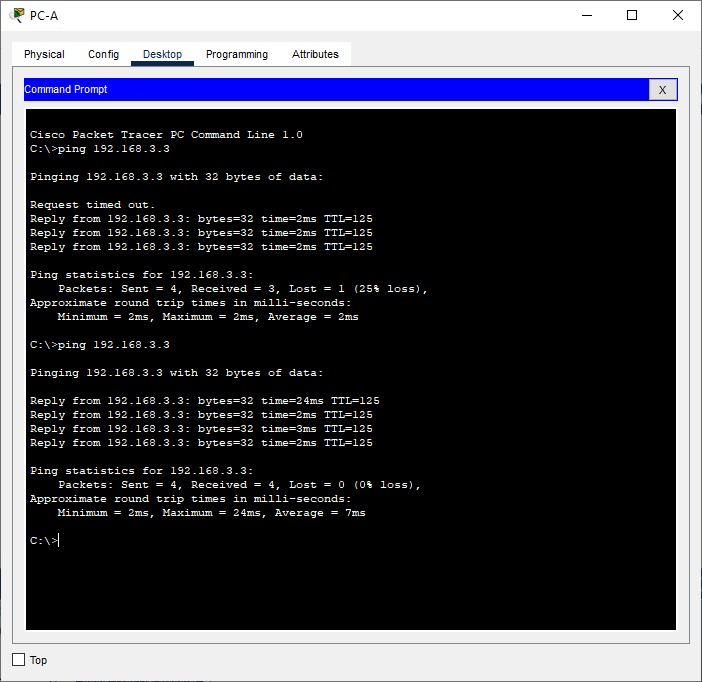
\includegraphics[scale=0.45]{img/task1-step1.png}
            \caption{Prueba de conectividad entre PC-C y PC-A}
            \label{fig:task1-step1}
        \end{figure}

        \begin{figure}[!h]
            \centering
            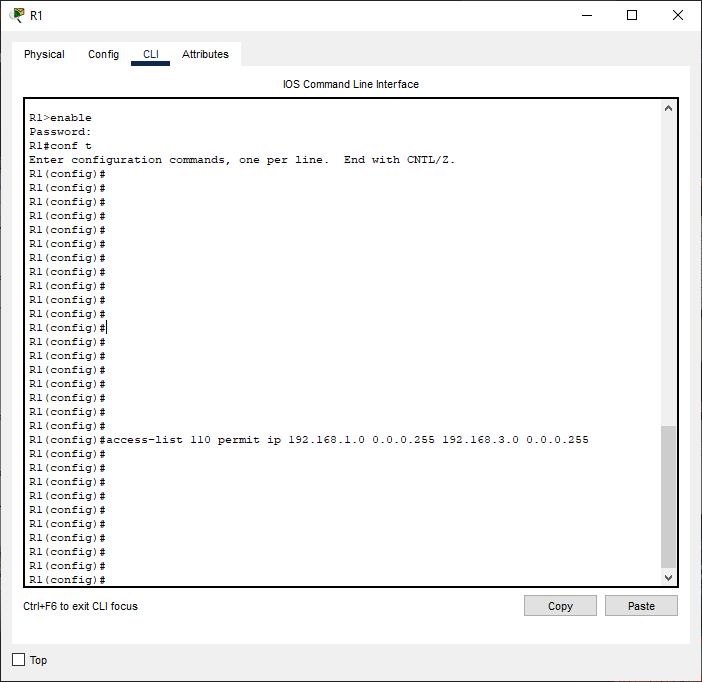
\includegraphics[scale=0.45]{img/task1-step2.png}
            \caption{Identificación de tráfico interesante en Router 1}
            \label{fig:task1-step2}
        \end{figure}

        \clearpage
        \begin{figure}[!h]
            \centering
            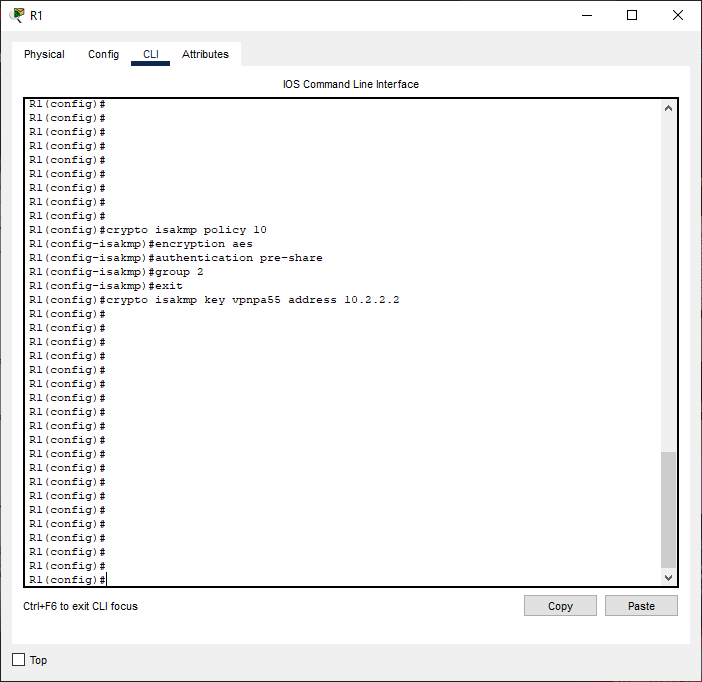
\includegraphics[scale=0.45]{img/task1-step3.png}
            \caption{Configuración de parámetros IPSec Fase 1 en Router 1}
            \label{fig:task1-step3}
        \end{figure}

        \begin{figure}[!h]
            \centering
            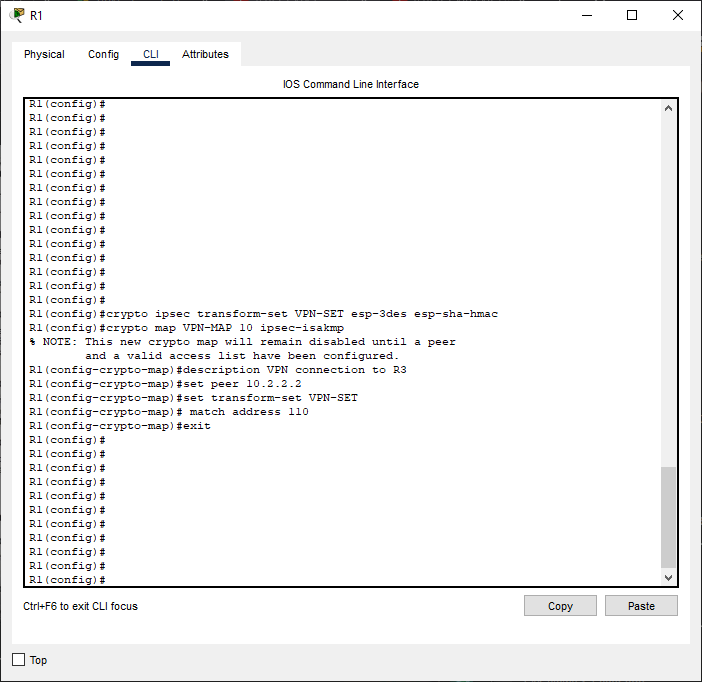
\includegraphics[scale=0.45]{img/task1-step4.png}
            \caption{Configuración de parámetros IPSec Fase 2 en Router 1}
            \label{fig:task1-step4}
        \end{figure}

        \clearpage
        \begin{figure}[!h]
            \centering
            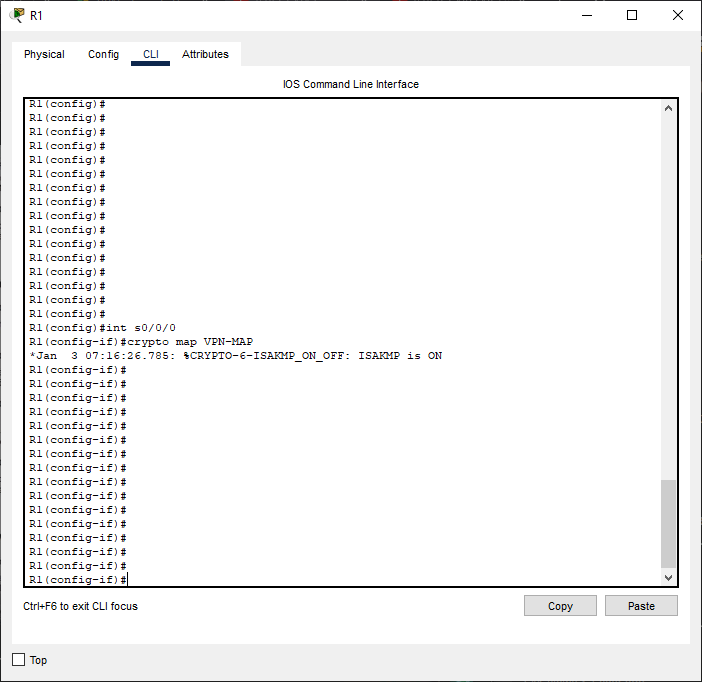
\includegraphics[scale=0.45]{img/task1-step5.png}
            \caption{Aplicación del \texttt{VPN-MAP} en la interfaz de salida de R1}
            \label{fig:task1-step5}
        \end{figure}

        \begin{figure}[!h]
            \centering
            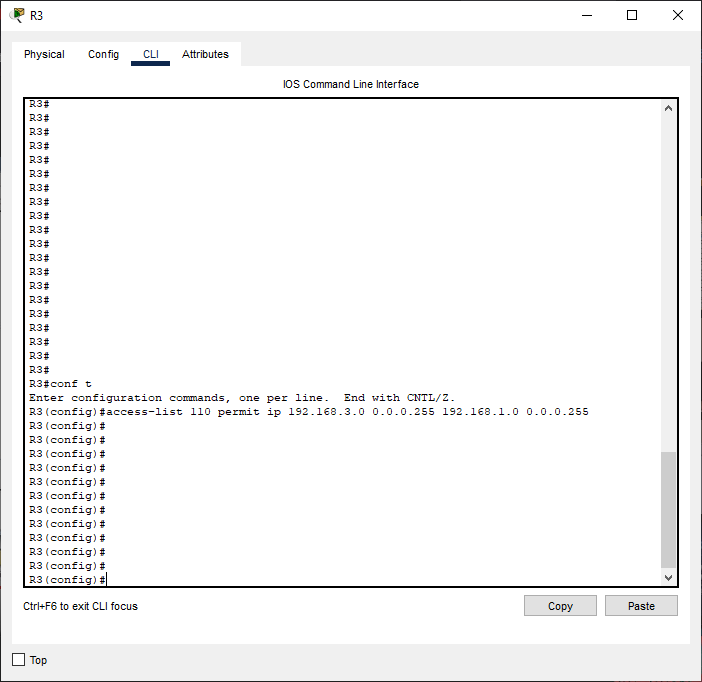
\includegraphics[scale=0.45]{img/task2-step1.png}
            \caption{Creación del \texttt{access-list} para la conexión a R1}
            \label{fig:task2-step1}
        \end{figure}

        \clearpage
        \begin{figure}[!h]
            \centering
            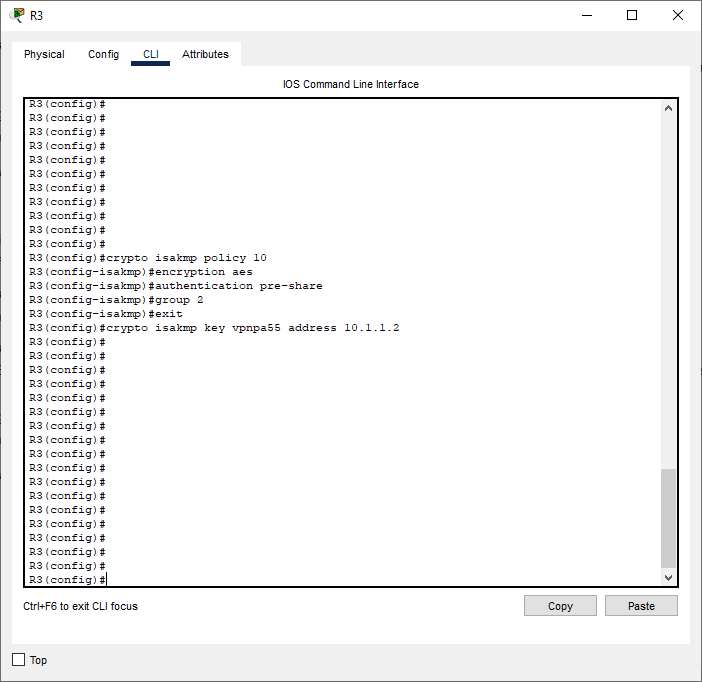
\includegraphics[scale=0.45]{img/task2-step2.png}
            \caption{Configuración de parámetros IPSec Fase 1 en Router 3}
            \label{fig:task2-step2}
        \end{figure}
        
        \begin{figure}[!h]
            \centering
            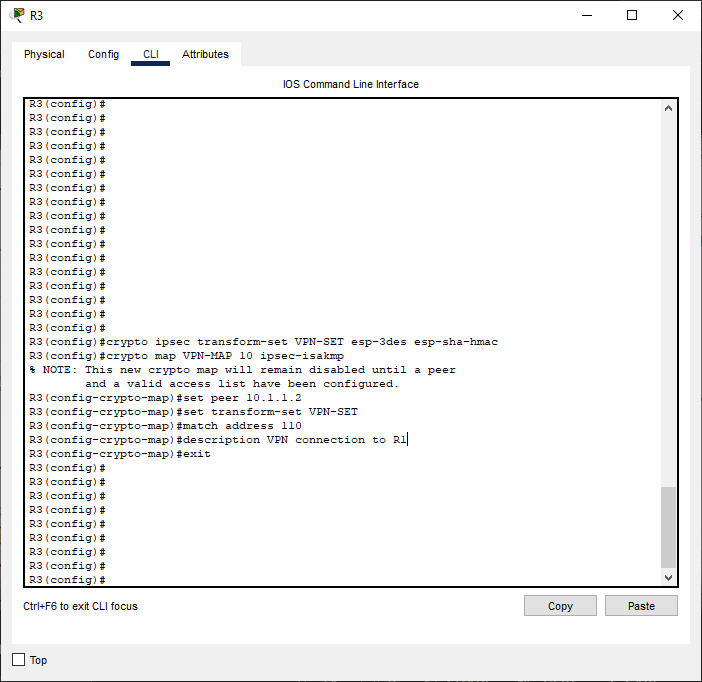
\includegraphics[scale=0.45]{img/task2-step3.png}
            \caption{Configuración de parámetros IPSec Fase 2 en Router 3}
            \label{fig:task2-step3}
        \end{figure}

        \clearpage
        \begin{figure}[!h]
            \centering
            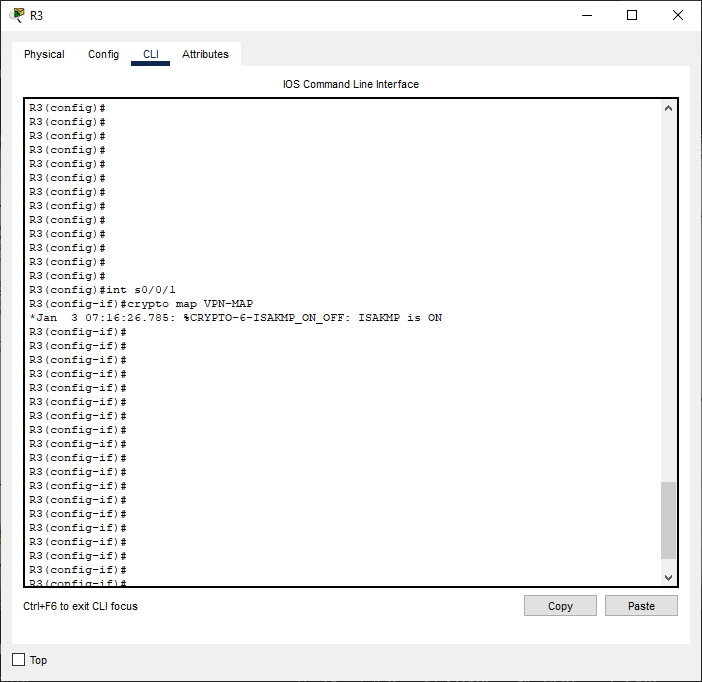
\includegraphics[scale=0.45]{img/task2-step4.png}
            \caption{Aplicación del \texttt{VPN-MAP} en la interfaz de salida de R3}
            \label{fig:task2-step4}
        \end{figure}

        \begin{figure}[!h]
            \centering
            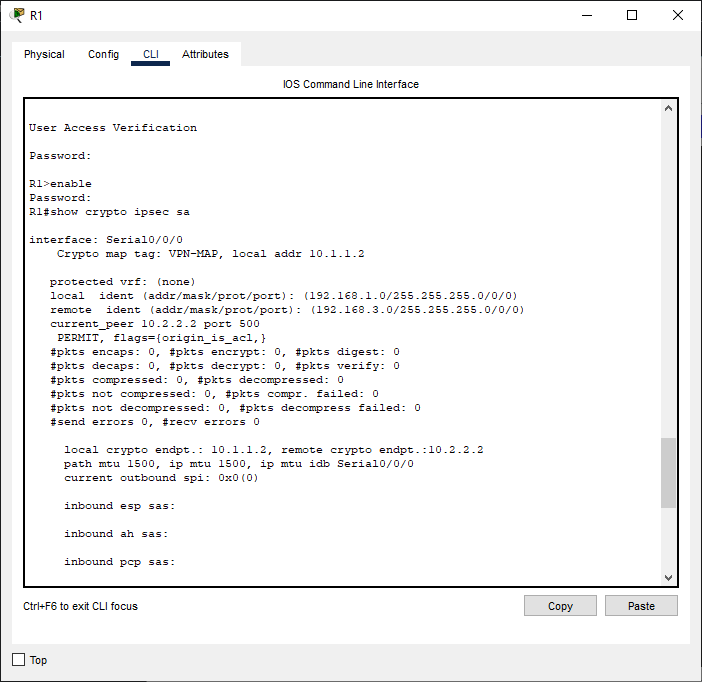
\includegraphics[scale=0.45]{img/task3-step1.png}
            \caption{Verificación de paquetes encriptados que hayan fluido por R1}
            \label{fig:task3-step1}
        \end{figure}

        \clearpage
        \begin{figure}[!h]
            \centering
            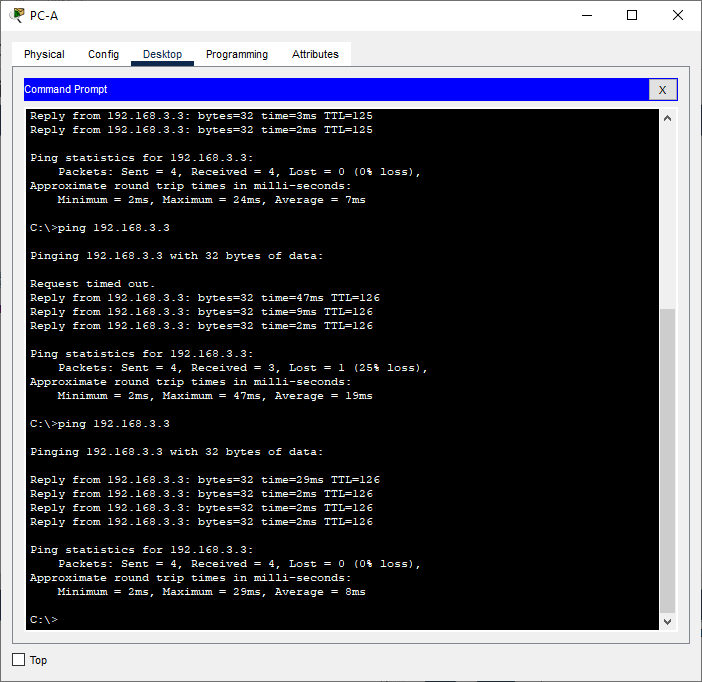
\includegraphics[scale=0.45]{img/task3-step2.png}
            \caption{Creación de tráfico interesante por R1}
            \label{fig:task3-step2}
        \end{figure}

        \begin{figure}[!h]
            \centering
            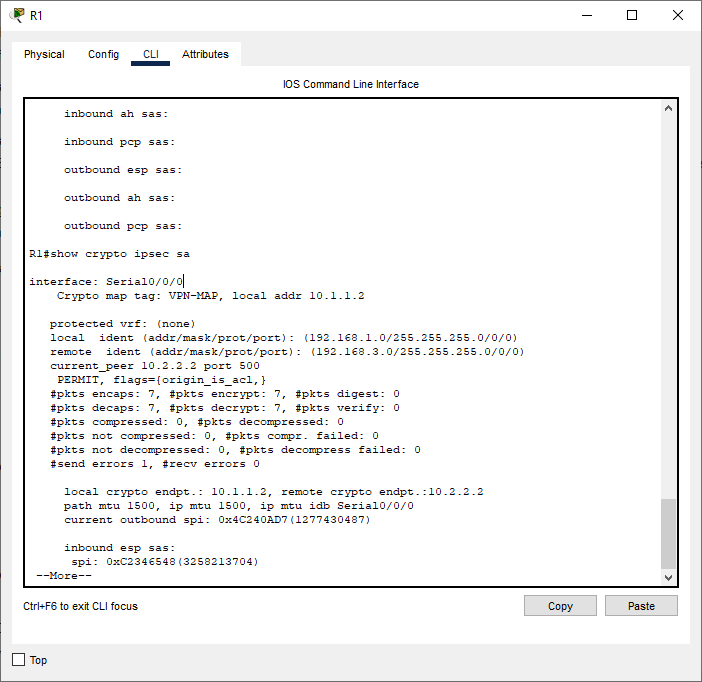
\includegraphics[scale=0.45]{img/task3-step3.png}
            \caption{Verificación de paquetes interesantes a través de R1 después de tráfico interesante}
            \label{fig:task3-step3}
        \end{figure}

        \clearpage
        \begin{figure}[!h]
            \centering
            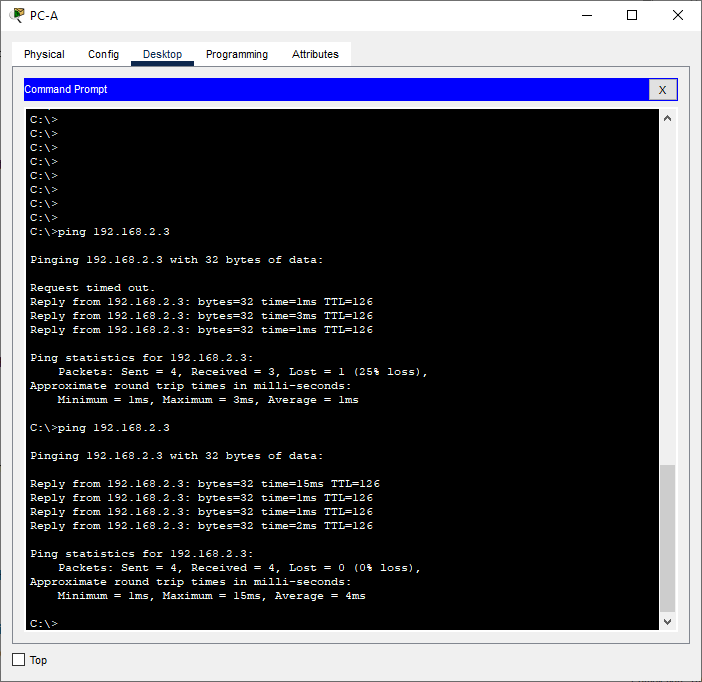
\includegraphics[scale=0.45]{img/task3-step4.png}
            \caption{Creación de tráfico no interesante por R1}
            \label{fig:task3-step4}
        \end{figure}

        \begin{figure}[!h]
            \centering
            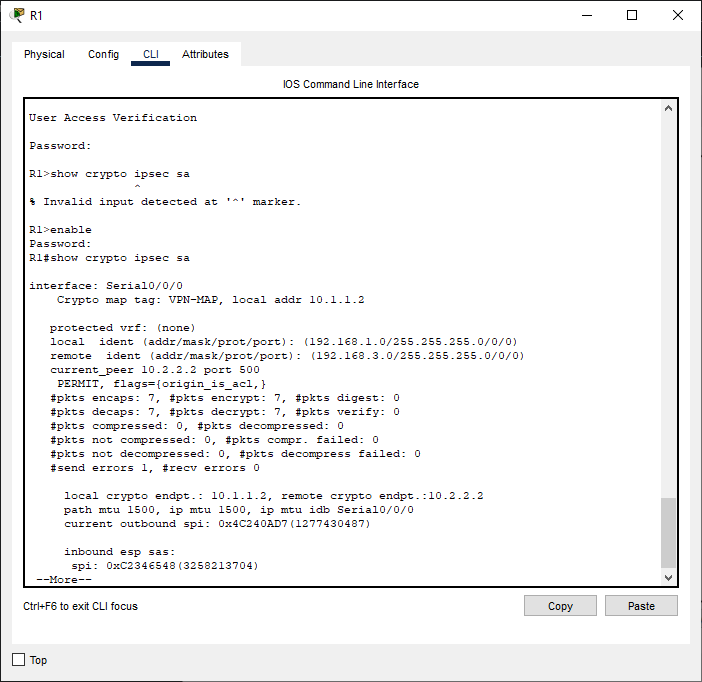
\includegraphics[scale=0.45]{img/task3-step5.png}
            \caption{Verificación de paquetes interesantes a través de R1 después del tráfico no interesante}
            \label{fig:task3-step5}
        \end{figure}

        \clearpage
        \begin{landscape}
            \begin{figure}[!h]
                \centering
                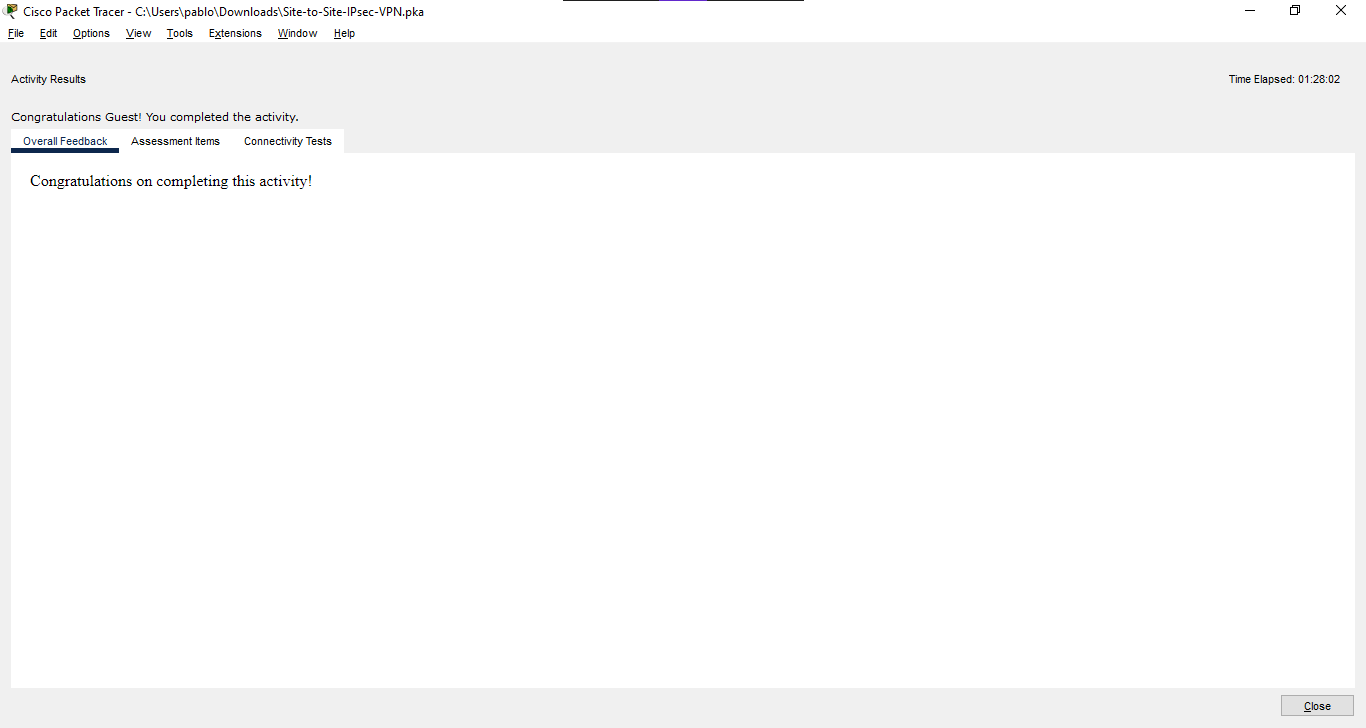
\includegraphics[scale=0.6]{img/task-completed.png}
                \caption{Evidencia de finalización de actividad}
                \label{fig:task-completed}
            \end{figure}
        \end{landscape}

\end{document}
